\section{Assessment of Data vs MC Before Unfolding}
\label{sec:GBJ2:Uncorr}
This section presents the data compared to the reconstructed PYTHIA sample.
Figures \ref{GBJ2:Uncorr:Incl_Gap} -- \ref{GBJ2:Uncorr:Q0} show the uncorrected data compared to PYTHIA.
The PYTHIA error bands are the quadrature sum of the statistical error and the JES uncertainty bands. 

Figure \ref{GBJ2:Uncorr:Incl_Gap} shows (a) the gap fraction and (b) the mean number of jets in the region bounded by the dijet system, as a function of \dy{}.
The gap fraction measured from data falls as a function of \dy{}, up to $\dy{}>5.5$ where it starts to level off.
The PYTHIA gap fraction curve is consistently below the data up to a $\dy{}=6.5$.
PYTHIA then rises for the larges \dy{} bins, and has a higher gap fraction for $\dy{}>7$. 
The mean multiplicity of jets in the rapidity region increases as a function of \dy{}, to a peak of about $1.2$ at $\dy{}=7$, and then plateaus.
Both the flattening out of the gap fraction and the plateau in the mean number of jets could be due to PDF effects, such as those seen in the previous analysis for dijets with large \dy{} and \ptb{}.


Figures \ref{GBJ2:Uncorr:dphi23}, \ref{GBJ2:Uncorr:dphi45}, and \ref{GBJ2:Uncorr:dphi78} show \dphidyDist{} for $2<\dy{}<3$, $4<\dy{}<5$, and $7<\dy{}<8$,  respectively, for (a) inclusive events and (b) gap events.
PYTHIA does not describe the data particularly well, especially at high \dphi{} for  $2<\dy{}<3$ and $4<\dy{}<5$ slices where it is about $20\%$ below the data.
In the  $7<\dy{}<8$ slice, the PYTHIA results are still consistently below the data, but they agree within the JES uncertainty band.
The cross-section from PYTHIA does not agree with the measured cross-section, as there are large uncertainties in the leading order plus leading logarithm cross-section used by PYTHIA.

Figures \ref{GBJ2:Uncorr:cos} and \ref{GBJ2:Uncorr:cos2} show the \mean{\cosdphi{}} and \mean{\costwodphi{}} variables respectively, as a function of the dijet separation, \dy{}, for (a) inclusive and (b) gap events.
A \mean{\cosdphi{}} value of 1 corresponds to perfectly back-to-back jets in azimuth.
The \mean{\cosdphi{}} distribution for the inclusive events have a value of about $0.94$ for $\dy{}<2$.
As the $\dy{}$ increases, the jets become less back-to-back and the value of \mean{\cosdphi{}} falls and then levels off at a value of about $0.86$ for $\dy{}=6$.
As the $\dy{}$ increases, the available phase space to emit into is larger due to the jets being at very high energies.
For the gap events, the \mean{\cosdphi{}} at low \dy{} starts at a similar level to the inclusive events, but then slowly rises to a maximum of about $0.96$.
When the \dy{} is low, emissions can fall outside the rapidity region, but as the \dy{} increases this region becomes smaller, and the jet veto is stopping hard emission into the rapidity region, thus the dijets are more back-to-back.
The PYTHIA distribution show a slightly different shape from the data.
At both low and high \dy{}, the \mean{\cosdphi{}} for PYTHIA is higher than the data for both gap and inclusive events. 
In the range $2<\dy{}<5.5$, PYTHIA describes the data well.
The shape of the \mean{\costwodphi{}} distribution has a similar explanation to the \mean{\cosdphi{}} distribution, and shows similar features.
For both inclusive and gap events, PYTHIA's description of \mean{\costwodphi{}} is too low at low \dy{} and too high at high \dy{}.

Figure \ref{GBJ2:Uncorr:Q0} shows the gap fraction as a function of the jet veto scale, \qz{}, for the \dy{} ranges $2<\dy{}<3$, $4<\dy{}<5$, and $7<\dy{}<8$.
As \qz{} is increased, fewer events are defined as gap events, until at high \qz{} the gap fraction is at $1.0$.
In the range $2<\dy{}<3$, the PYTHIA gap fraction is lower than the data for $\qz{}<50$ GeV, though it is within the JES uncertainty.
In the range $4<\dy{}<5$, the PYTHIA gap fraction describes the data well for the full \qz{} range.
For dijets within the range $7<\dy{}<8$, the PYTHIA gap fraction is higher than the data until both gap fractions plateau at $1.0$.

\begin{figure}
\centering
        \begin{subfigure}[b]{0.5\textwidth}
                \centering
                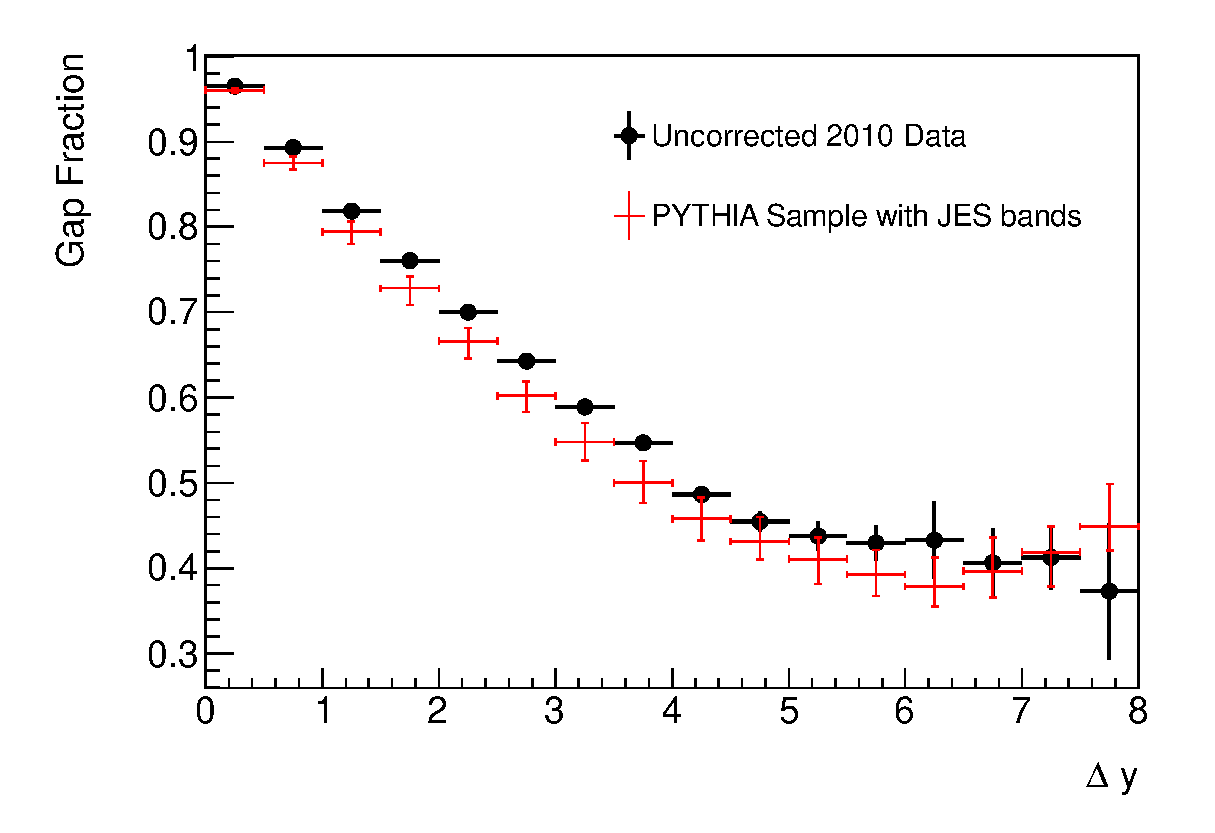
\includegraphics[width=\textwidth]{figures/GBJ2/ControlPlots/Smeared__GapFraction_deltaY.eps}
        \end{subfigure}%
        \begin{subfigure}[b]{0.5\textwidth}
                \centering
                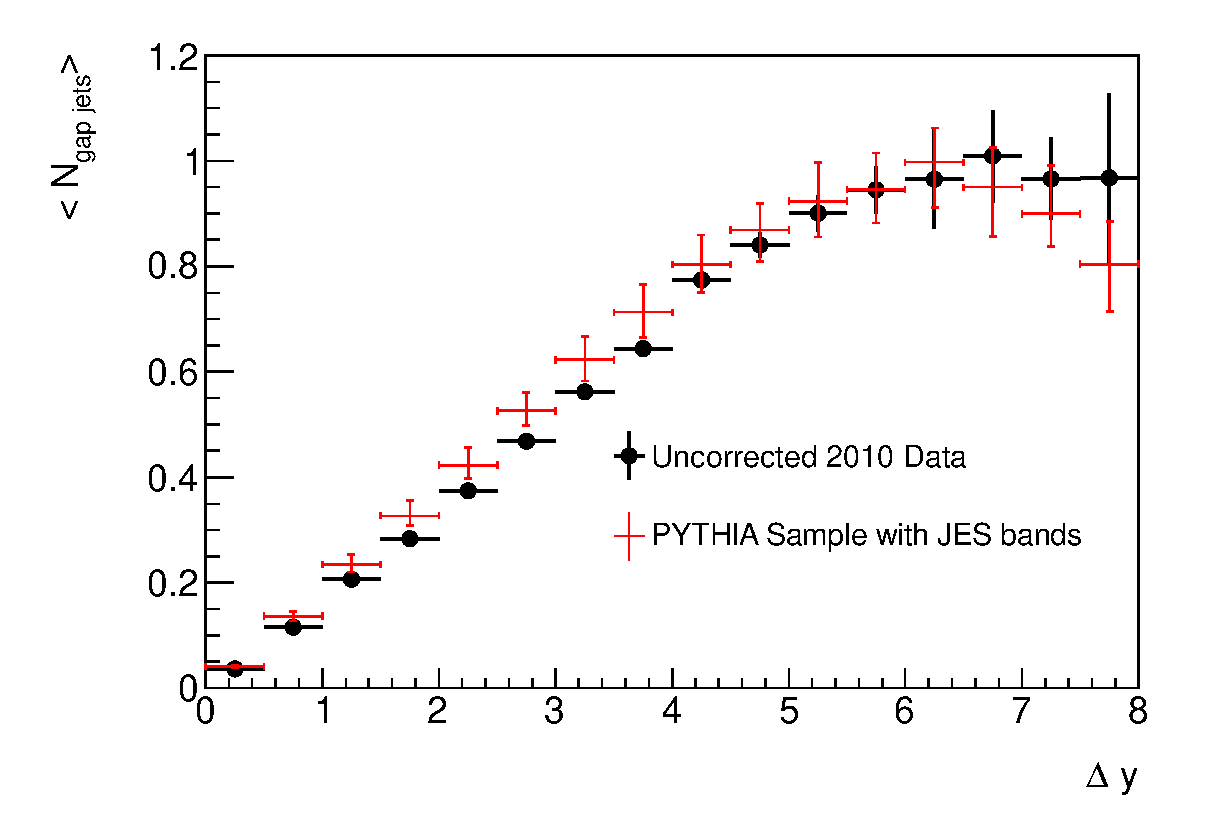
\includegraphics[width=\textwidth]{figures/GBJ2/ControlPlots/Smeared__prof_deltaY_njets.eps}
        \end{subfigure}%
\caption[Comparison of the data and PYTHIA for the gap fraction and mean number of jets]{
(a) The gap fraction  and (b) the mean number of jets in the rapidity region bounded by the dijet system as a function of \dy{} for 2010 uncorrected data (black points) and reconstructed PYTHIA sample (red points).
\label{GBJ2:Uncorr:Incl_Gap}}
\end{figure}



\begin{figure}
\centering
        \begin{subfigure}[b]{0.5\textwidth}
                \centering
                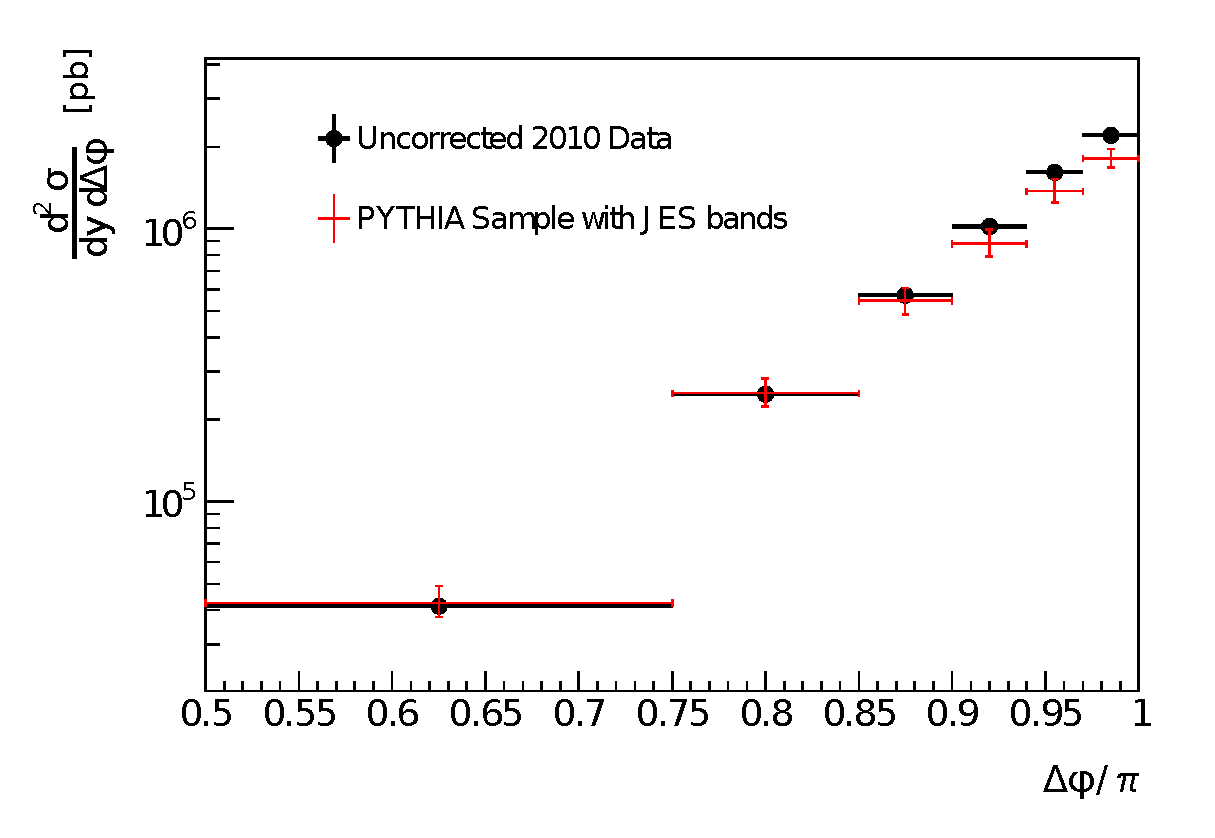
\includegraphics[width=\textwidth]{figures/GBJ2/ControlPlots/Smeared__dPhi__2_3.eps}
        \end{subfigure}%
        \begin{subfigure}[b]{0.5\textwidth}
                \centering
                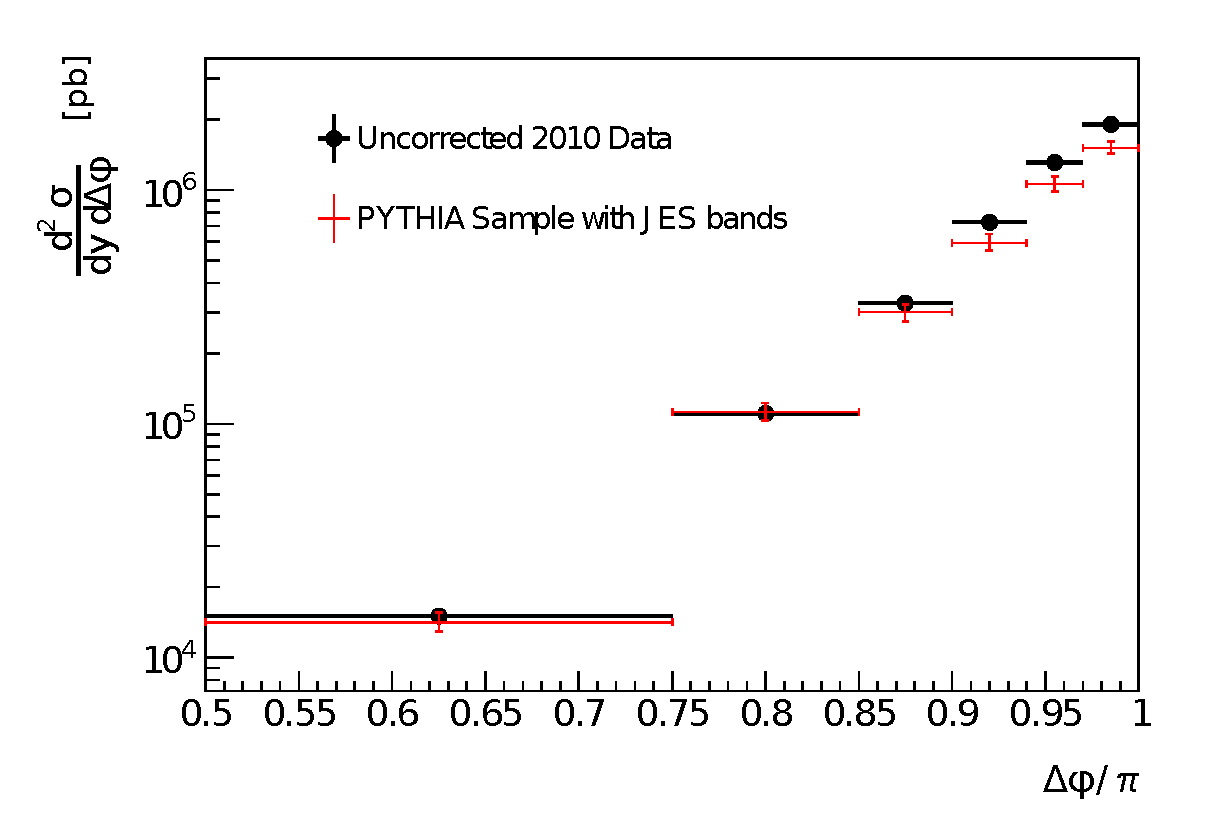
\includegraphics[width=\textwidth]{figures/GBJ2/ControlPlots/Smeared__dPhi_gap__2_3.eps}
        \end{subfigure}%
\caption[Comparison of the data and PYTHIA for \dphidyDist{} with $2<\dy{}<3$]{
\dphidyDist{} for (a) inclusive events and (b) gap events for a dijet separation, \dy{} of 2-3 for 2010 uncorrected data (black points) and reconstructed PYTHIA sample (red points).
\label{GBJ2:Uncorr:dphi23}}
\end{figure}


\begin{figure}
\centering
        \begin{subfigure}[b]{0.5\textwidth}
                \centering
                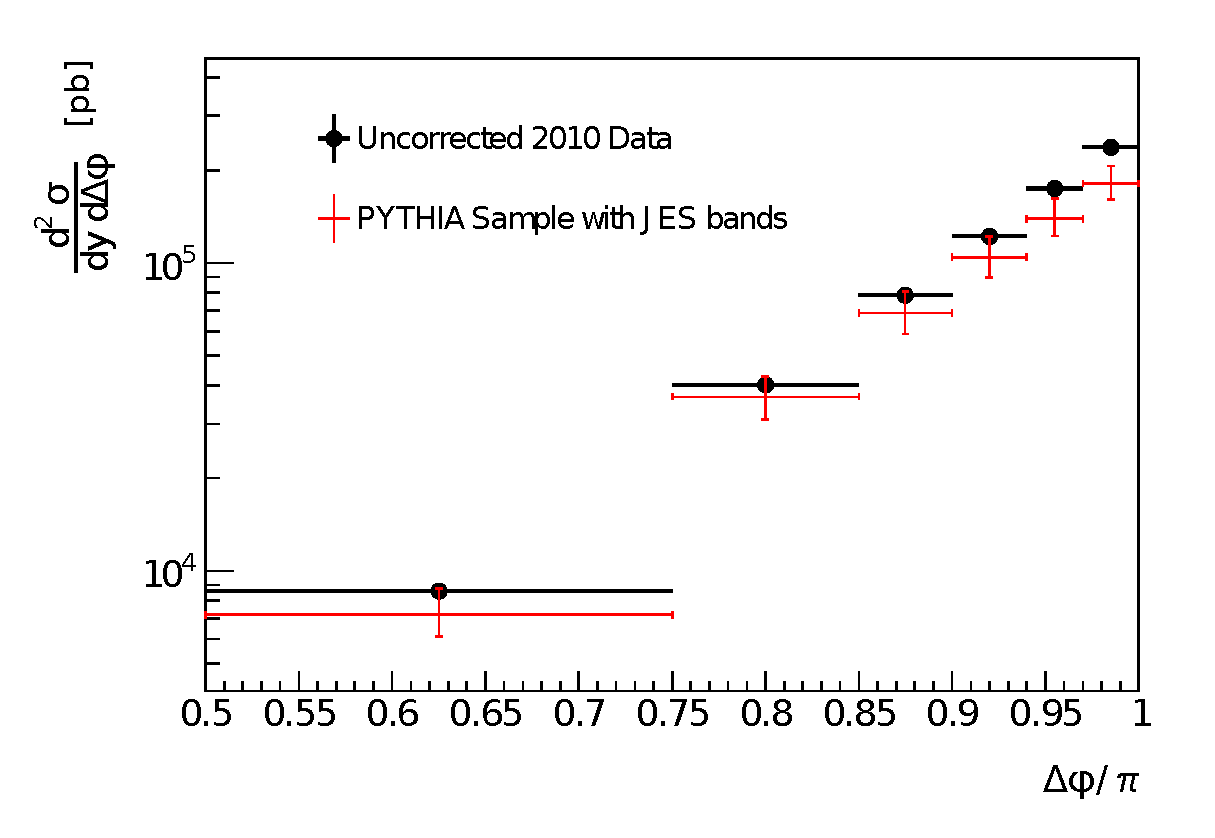
\includegraphics[width=\textwidth]{figures/GBJ2/ControlPlots/Smeared__dPhi__4_5.eps}
        \end{subfigure}%
        \begin{subfigure}[b]{0.5\textwidth}
                \centering
                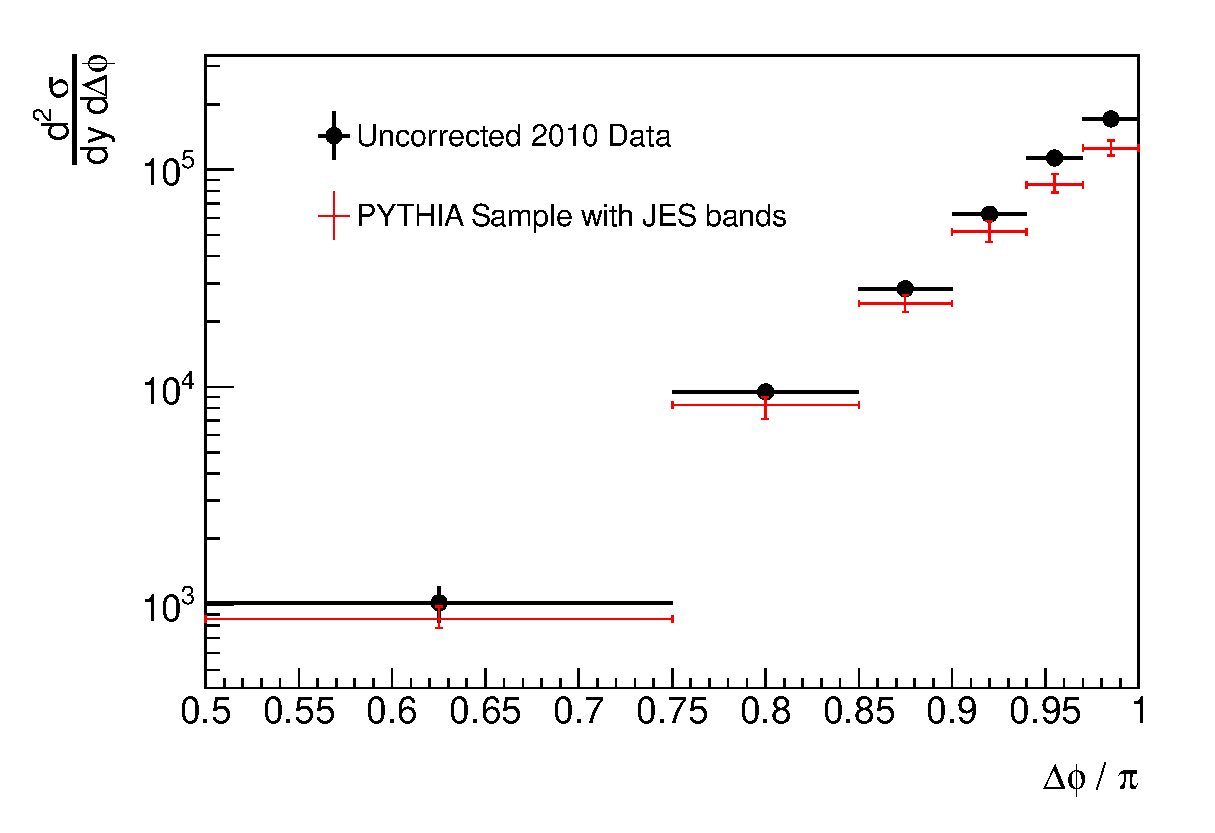
\includegraphics[width=\textwidth]{figures/GBJ2/ControlPlots/Smeared__dPhi_gap__4_5.eps}
        \end{subfigure}%
\caption[Comparison of the data and PYTHIA for \dphidyDist{} with $4<\dy{}<5$]{
\dphidyDist{} for (a) inclusive events and (b) gap events for a dijet separation, \dy{} of 4-5 for 2010 uncorrected data (black points) and reconstructed PYTHIA sample (red points).
\label{GBJ2:Uncorr:dphi45}}
\end{figure}



\begin{figure}
\centering
        \begin{subfigure}[b]{0.5\textwidth}
                \centering
                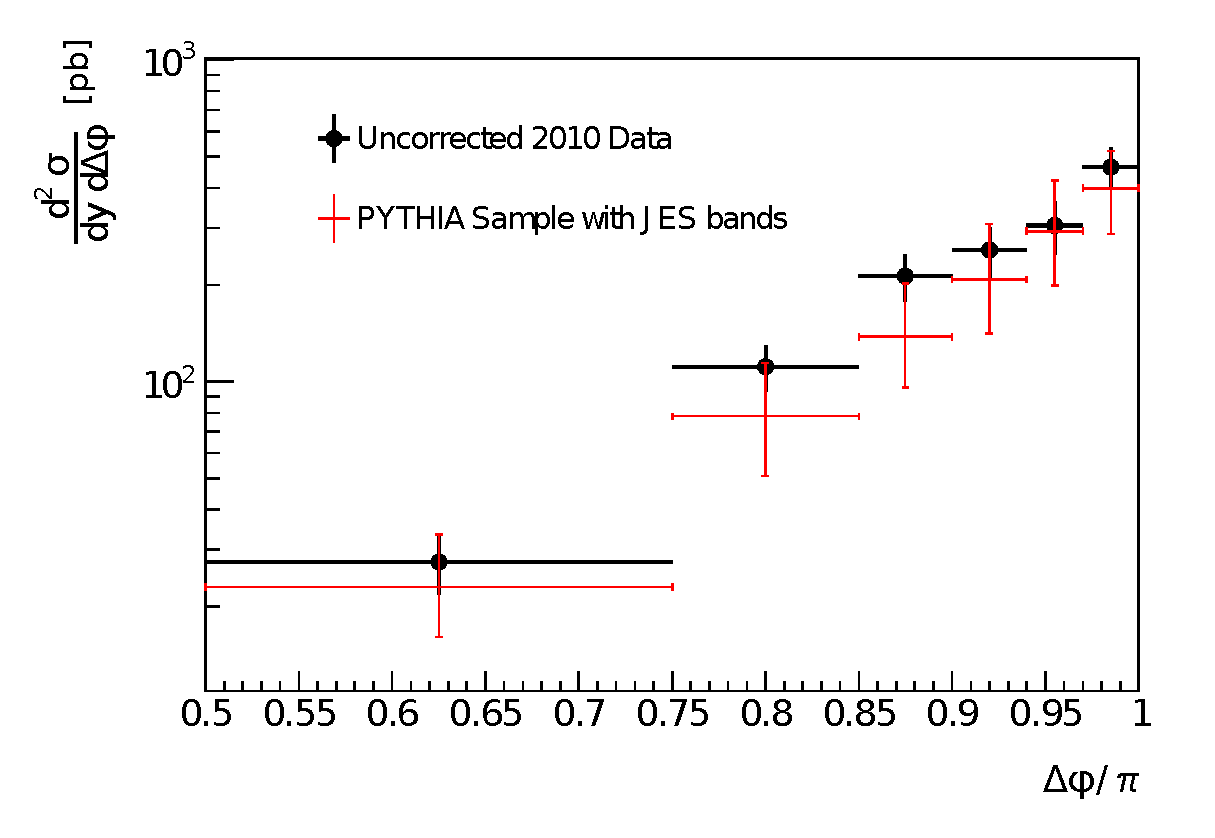
\includegraphics[width=\textwidth]{figures/GBJ2/ControlPlots/Smeared__dPhi__7_8.eps}
        \end{subfigure}%
        \begin{subfigure}[b]{0.5\textwidth}
                \centering
                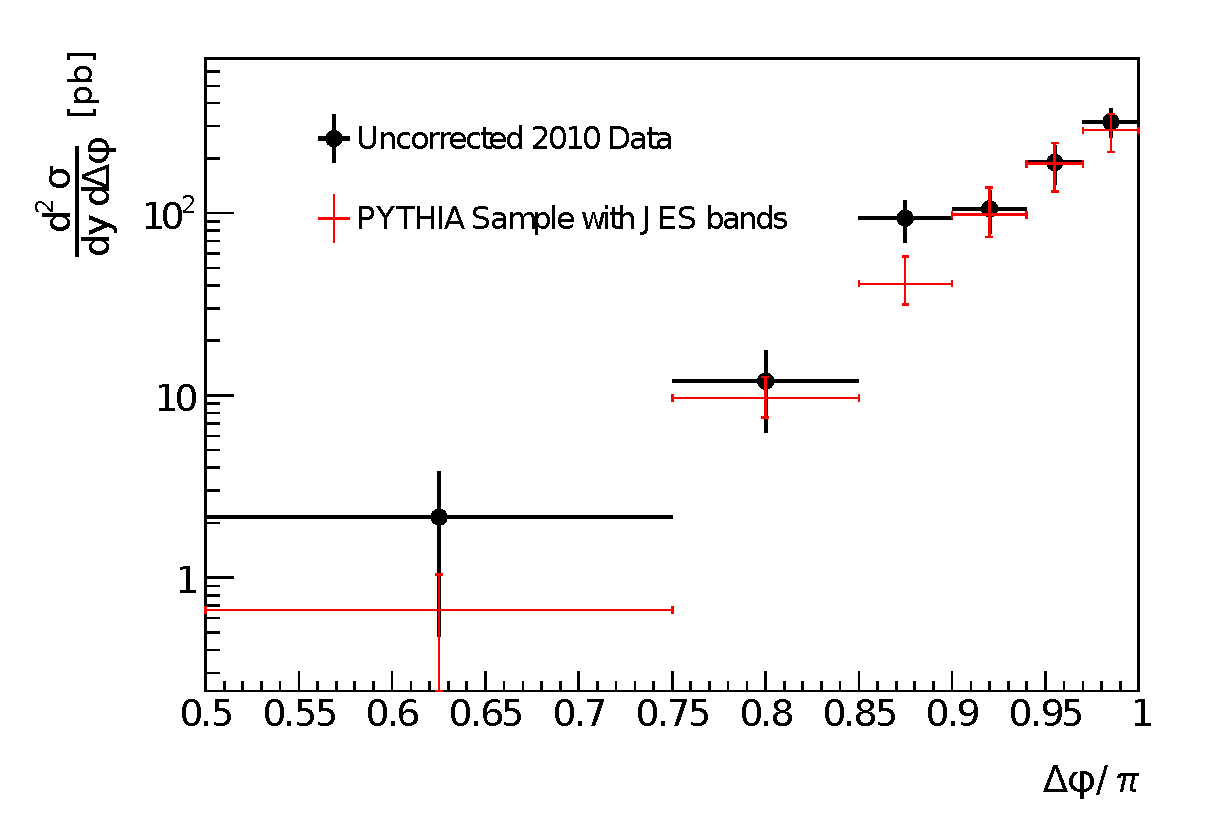
\includegraphics[width=\textwidth]{figures/GBJ2/ControlPlots/Smeared__dPhi_gap__7_8.eps}
        \end{subfigure}%
\caption[Comparison of the data and PYTHIA for \dphidyDist{} with $7<\dy{}<8$]{
\dphidyDist{} for (a) inclusive events and (b) gap events for a dijet separation, \dy{} of 7-8 for 2010 uncorrected data (black points) and reconstructed PYTHIA sample (red points).
\label{GBJ2:Uncorr:dphi78}}
\end{figure}



\begin{figure}
\centering
        \begin{subfigure}[b]{0.5\textwidth}
                \centering
                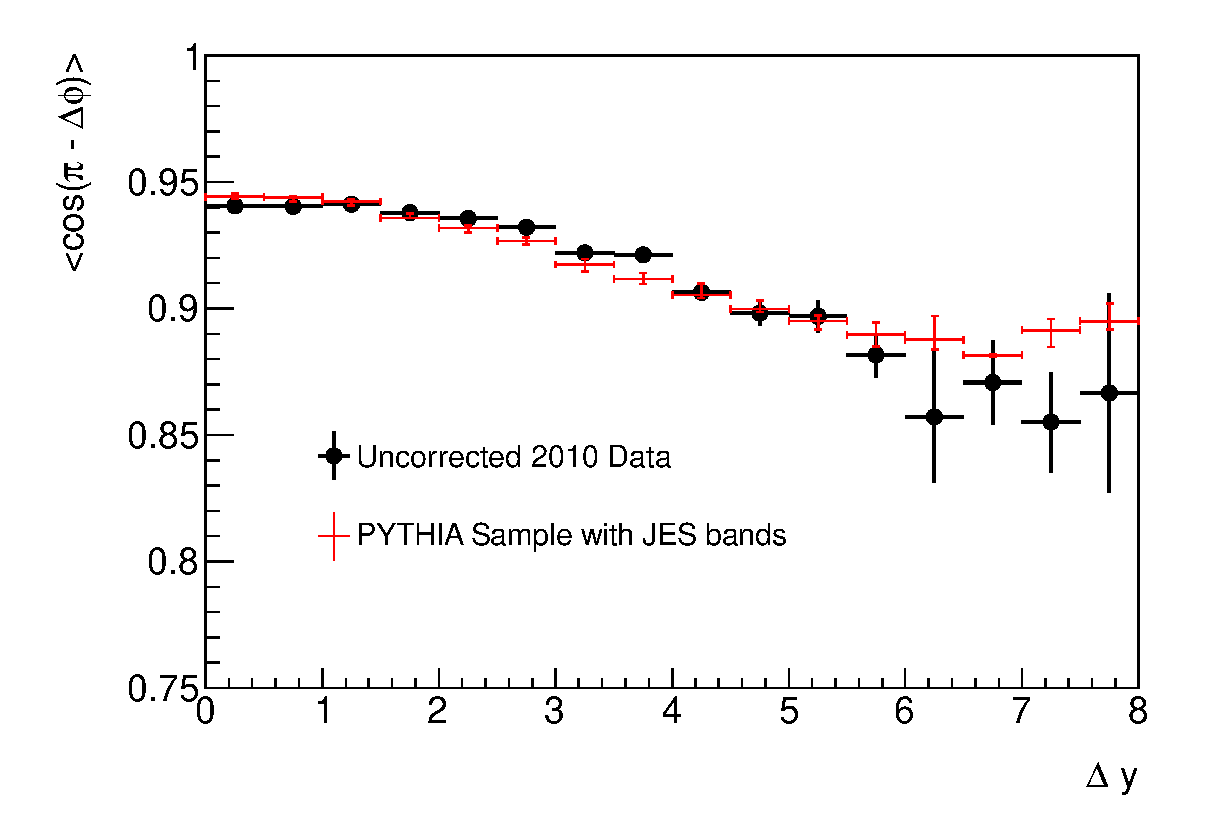
\includegraphics[width=\textwidth]{figures/GBJ2/ControlPlots/Smeared__cosdPhi_deltaY.eps}
        \end{subfigure}%
        \begin{subfigure}[b]{0.5\textwidth}
                \centering
                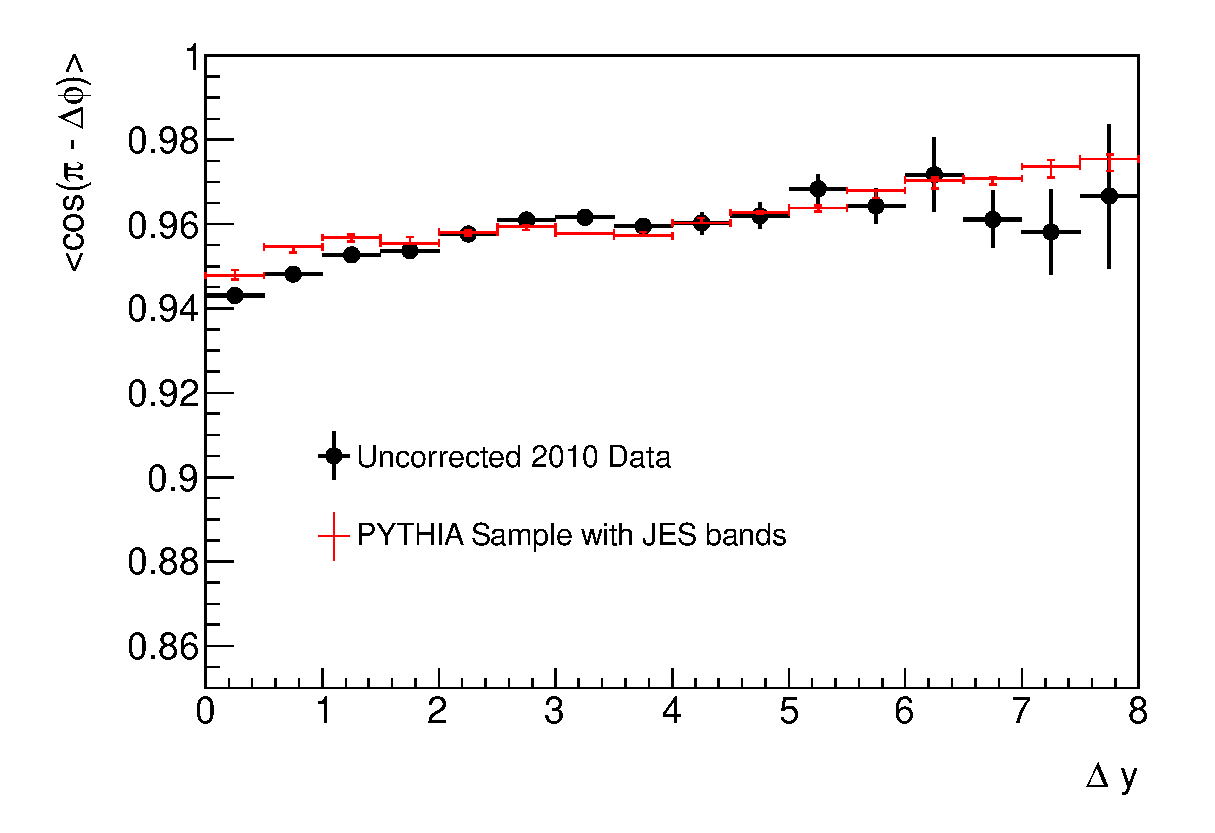
\includegraphics[width=\textwidth]{figures/GBJ2/ControlPlots/Smeared__cosdPhi_deltaY_gap.eps}
        \end{subfigure}%
\caption[Comparison of the data and PYTHIA for \cosdphi{}]{
\mean{\cosdphi{}} as a function of \dy{} for (a) inclusive and (b) gap events for 2010 uncorrected data (black points) and reconstructed PYTHIA sample (red points).
\label{GBJ2:Uncorr:cos}}
\end{figure}


\begin{figure}
\centering
        \begin{subfigure}[b]{0.5\textwidth}
                \centering
                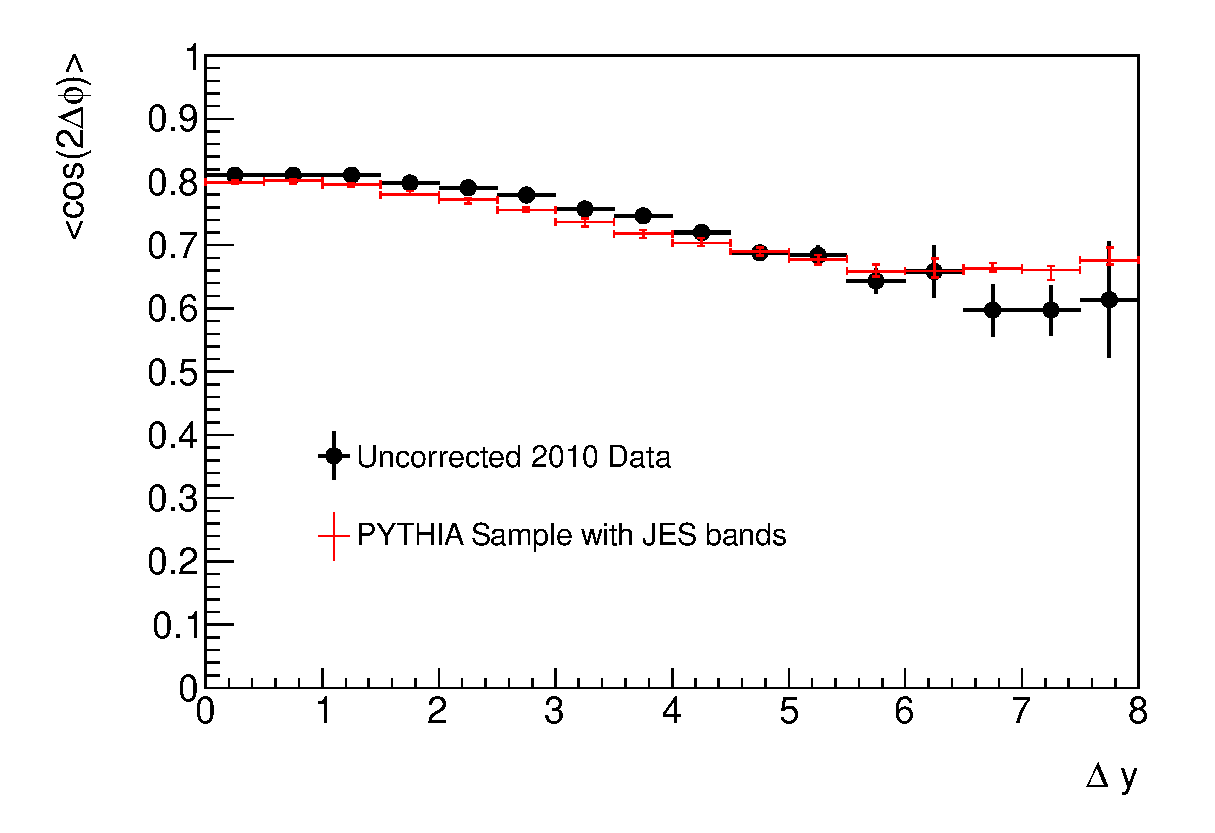
\includegraphics[width=\textwidth]{figures/GBJ2/ControlPlots/Smeared__cos2dPhi_deltaY.eps}
        \end{subfigure}%
        \begin{subfigure}[b]{0.5\textwidth}
                \centering
                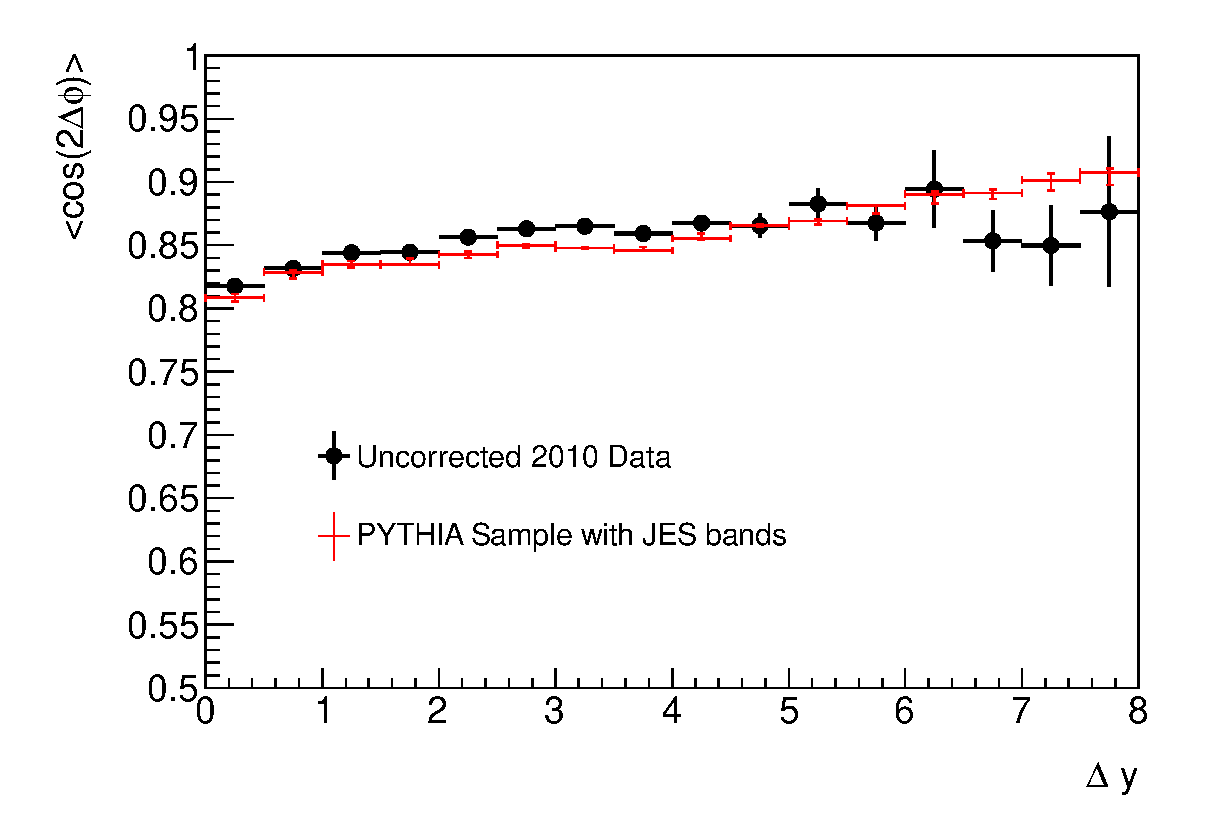
\includegraphics[width=\textwidth]{figures/GBJ2/ControlPlots/Smeared__cos2dPhi_deltaY_gap.eps}
        \end{subfigure}%
\caption[Comparison of the data and PYTHIA for \costwodphi{}]{
\mean{\costwodphi{}} as a function of \dy{} for (a) inclusive and (b) gap events for 2010 uncorrected data (black points) and reconstructed PYTHIA sample (red points).
\label{GBJ2:Uncorr:cos2}}
\end{figure}

\begin{figure}
\centering
        \begin{subfigure}[b]{0.5\textwidth}
                \centering
                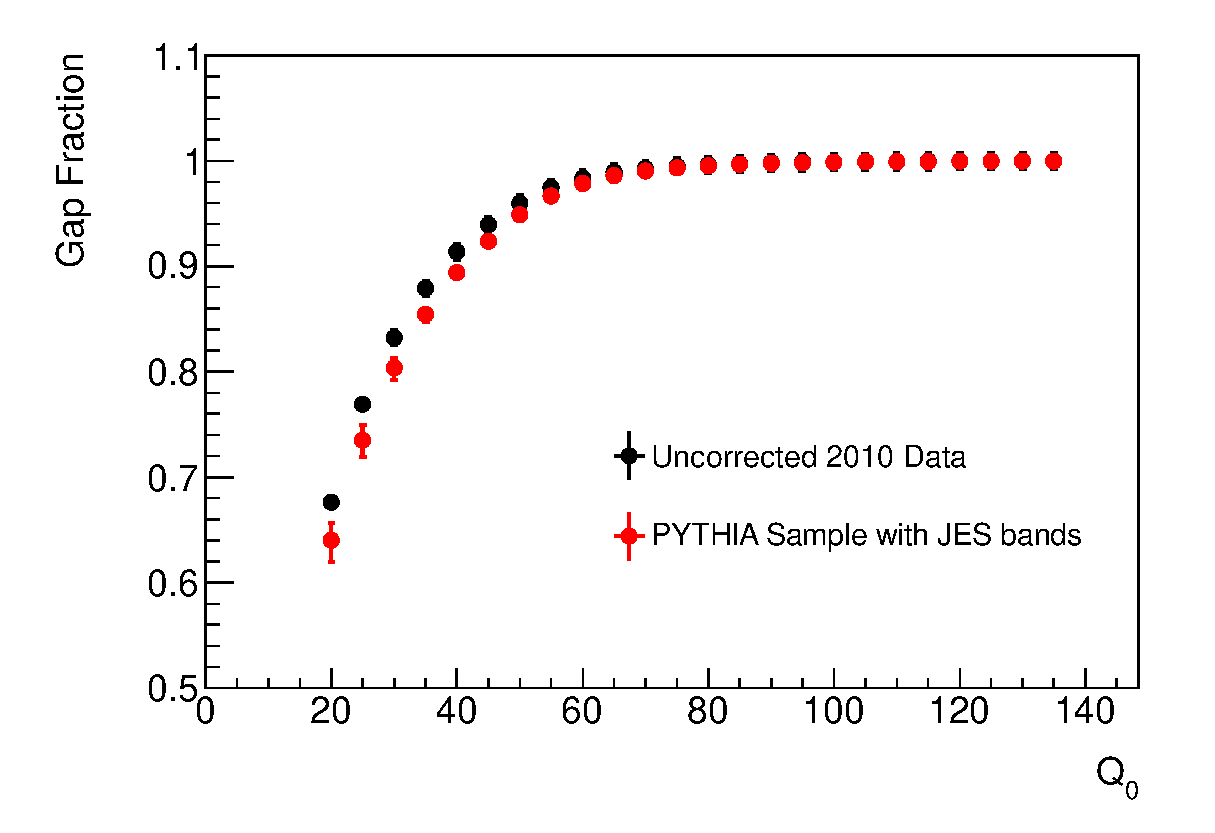
\includegraphics[width=\textwidth]{figures/GBJ2/ControlPlots/Smeared2_3__Q0.eps}
        \end{subfigure}%
        \begin{subfigure}[b]{0.5\textwidth}
                \centering
                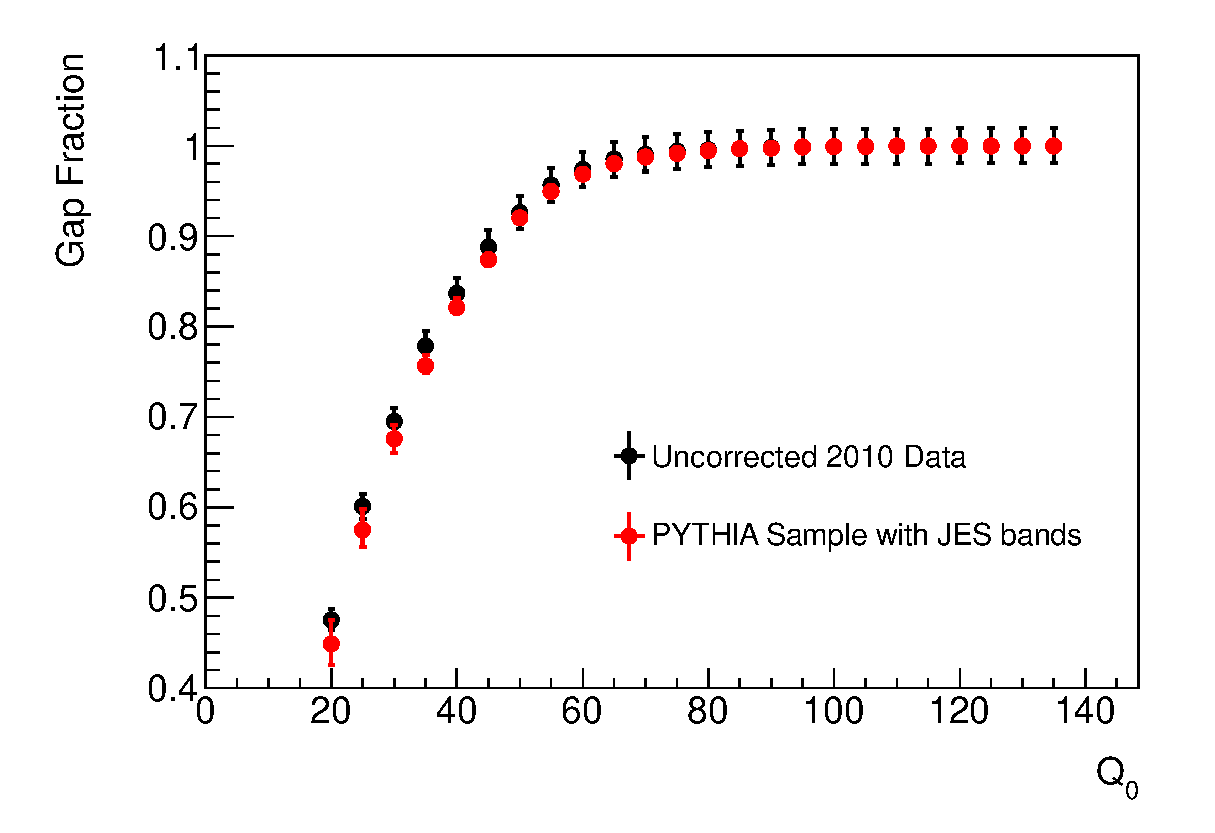
\includegraphics[width=\textwidth]{figures/GBJ2/ControlPlots/Smeared4_5__Q0.eps}
        \end{subfigure}%


        \begin{subfigure}[b]{0.5\textwidth}
                \centering
                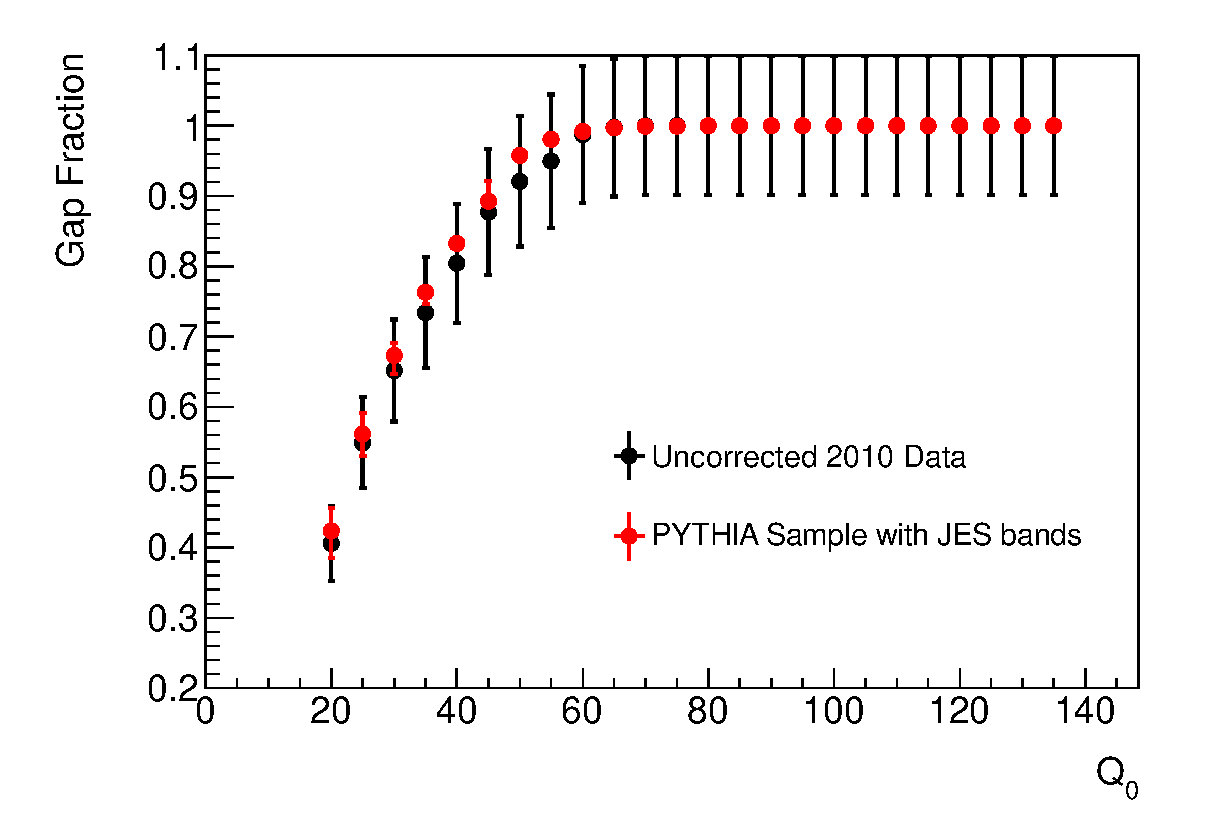
\includegraphics[width=\textwidth]{figures/GBJ2/ControlPlots/Smeared7_8__Q0.eps}
        \end{subfigure}%
\caption[Comparison of the data and PYTHIA for the gap fraction as a function of \qz{}]{
The gap fraction against \qz{} for (a) $2<\dy{}<3$, (b) $4<\dy{}<5$ and (c) $7<\dy{}<8$ for 2010 uncorrected data (black points) and reconstructed PYTHIA sample (red points).
\label{GBJ2:Uncorr:Q0}}
\end{figure}

